%%%%%%%%%%%%%%%%%%%%%%%%%%%%%%%%%%%%%%%%%
% Beamer Presentation
% LaTeX Template
% Version 1.0 (10/11/12)
%
% This template has been downloaded from:
% http://www.LaTeXTemplates.com
%
% License:
% CC BY-NC-SA 3.0 (http://creativecommons.org/licenses/by-nc-sa/3.0/)
%
%%%%%%%%%%%%%%%%%%%%%%%%%%%%%%%%%%%%%%%%%

%----------------------------------------------------------------------------------------
%   PACKAGES AND THEMES
%----------------------------------------------------------------------------------------
\documentclass{beamer}

\newcounter{saveenumi}
\newcommand{\seti}{\setcounter{saveenumi}{\value{enumi}}}
\newcommand{\conti}{\setcounter{enumi}{\value{saveenumi}}}


%\usepackage{enumitem}
\mode<presentation> {

% The Beamer class comes with a number of default slide themes
% which change the colors and layouts of slides. Below this is a list
% of all the themes, uncomment each in turn to see what they look like.

%\usetheme{default}
%\usetheme{AnnArbor}
%\usetheme{Antibes}
%\usetheme{Bergen}
%\usetheme{Berkeley}
%\usetheme{Berlin}
%\usetheme{Boadilla}
%\usetheme{CambridgeUS}
%\usetheme{Copenhagen}
%\usetheme{Darmstadt}
%\usetheme{Dresden}
%\usetheme{Frankfurt}
%\usetheme{Goettingen}
%\usetheme{Hannover}
\usetheme{Ilmenau}
%\usetheme{JuanLesPins}
%\usetheme{Luebeck}
%\usetheme{Madrid}
%\usetheme{Malmoe}
%\usetheme{Marburg}
%\usetheme{Montpellier}
%\usetheme{PaloAlto}
%\usetheme{Pittsburgh}
%\usetheme{Rochester}
%\usetheme{Singapore}
%\usetheme{Szeged}
%\usetheme{Warsaw}

% As well as themes, the Beamer class has a number of color themes
% for any slide theme. Uncomment each of these in turn to see how it
% changes the colors of your current slide theme.

%\usecolortheme{albatross}
%\usecolortheme{beaver}
%\usecolortheme{beetle}
%\usecolortheme{crane}
%\usecolortheme{dolphin}
%\usecolortheme{dove}
%\usecolortheme{fly}
%\usecolortheme{lily}
%\usecolortheme{orchid}
%\usecolortheme{rose}
%\usecolortheme{seagull}
%\usecolortheme{seahorse}
%\usecolortheme{whale}
%\usecolortheme{wolverine}

%\setbeamertemplate{footline} % To remove the footer line in all slides uncomment this line
%\setbeamertemplate{footline}[page number] % To replace the footer line in all slides with a simple slide count uncomment this line

%\setbeamertemplate{navigation symbols}{} % To remove the navigation symbols from the bottom of all slides uncomment this line
}

\usepackage{graphicx} % Allows including images
\usepackage{booktabs} % Allows the use of \toprule, \midrule and \bottomrule in tables

%\usepackage{enumitem}

%----------------------------------------------------------------------------------------
%   TITLE PAGE
%----------------------------------------------------------------------------------------

\title[Hmuan Olfaction]{Study of Human Olfaction Using fMRI} % The short title appears at the bottom of every slide, the full title is only on the title page

\author{A. Afsharrad, H. Hojjati, M. Kiani, B. Moniri} % Your name
\institute[Sharif University of Technology] % Your institution as it will appear on the bottom of every slide, may be shorthand to save space
{
Ambient Intelligence Research Lab (AIR Lab)\\ \textbf{Sharif University of Technology} \\ 
\medskip
 % Your email address
}

\date{\today} % Date, can be changed to a custom date

\begin{document}

\begin{frame}
\titlepage % Print the title page as the first slide
\end{frame}

\begin{frame}
\frametitle{Overview} % Table of contents slide, comment this block out to remove it
\tableofcontents % Throughout your presentation, if you choose to use \section{} and \subsection{} commands, these will automatically be printed on this slide as an overview of your presentation
\end{frame}

%----------------------------------------------------------------------------------------
%   PRESENTATION SLIDES
%----------------------------------------------------------------------------------------

%------------------------------------------------
\section{Introduction} 

\begin{frame}
\frametitle{Objectives}
\textbf{The Main Objective:}
a study of human olfaction and olfactory dysfunction detection (judical use)
\\
\vspace{0.5cm}

\textbf{Side Objectives:}
\begin{enumerate}
	\item
	decoding \emph{surprise} in an olfactory oddball task
	\item
	studying the effect of \emph{stimulus length} on brain signals
\end{enumerate}
Above methods are used to classify normal and dysfunctional olfaction
\end{frame}

%------------------------------------------------

\section{Literature Review} 

\begin{frame}
\frametitle{Literature Review - Stimulus Duration}

\begin{enumerate}
	\item \textrm{\textbf{Activation and Habituation in Olfaction}}
	\\
	Poellinger et al. (2001), NeuroImage.\\
	\begin{itemize}
		\item
		a study of olfactory stimulus duration effect on human BOLD response
	\end{itemize}

	\item  \textrm{\textbf{Olfactory fMRI: Implications of Stimulation Length and Repetition Time}}\\
	Georgiopoulos et al. (2018), Chemical Senses.\\
	
	\begin{itemize}
		\item
		Two stimulation lengths and two repititon times.
		\item
		plotting the event related time course of brain activation in the four olfactory regions of interest. 
	\end{itemize}
	\seti
\end{enumerate}
	

	


\end{frame}


\begin{frame}
\frametitle{Literature Review - Oddball Paradigm}
\begin{enumerate}
	\conti
	\item \textrm{\textbf{Neural Correlates of Olfactory Change Detection}}
	\\
	Merav Sabri et al. (2004), NeuroImage.
	\begin{itemize}
		\item
		a study of both passive and active detection of olfactory change
		\item
		fMRI and the common oddball paradigm
	\end{itemize}
	\item \textrm{\textbf{Detection of Olfactory Dysfunction Using Olfactory Event
			Related Potentials in Young Patients with Multiple
			Sclerosis}}
	\\
	Fabrizia Caminiti et al. (2014), PLOS ONE.
	\begin{itemize}
		\item
		detection of olfactory dysfunction 
		\item
		Olfactory Event Related Potentials (OERP signals) used (no fMRI)
	\end{itemize}
	\seti
\end{enumerate}
\end{frame}

\begin{frame}
\frametitle{Literature Review - Olfactometer}
\begin{enumerate}
	\conti
	\item \textrm{\textbf{A Computer-Controlled Olfactometer for fMRI and Electrophysiological Studies of Olfaction}}
	\\
	Tyler S.Lorig et al. (1999), Behavior Research Methods, Instruments, \& Computers.
	\begin{itemize}
		\item
		design for an inexpensive and reliable olfactometer
		\item
		computer-controlled odor administration
		\item
		no ferrous material near the subject (for fMRI use)
	\end{itemize}
	\item \textrm{\textbf{Methods for Building an Inexpensive Computer-Controlled Olfactometer for Temporary-Precise Experiments}}
	\\
	Johan N. Lundstr$\ddot{\textrm{o}}$m et al. (2010), International Journal of Psychophysiology.
	\begin{itemize}
		\item
		a complete guide for building an olfactometer suitable for behavioral experiments
	\end{itemize}
	
\end{enumerate}
\end{frame}



\section{Applications} 
\begin{frame}
	\frametitle{Significance and Application of Olfaction Study}
	\begin{enumerate}
		\item
		Diagnosis of Olfactory Dysfunction
		\begin{itemize}
			\item
			Judical use of malingering Detection
			\item 
			Early Diagnosis of Various Disorders
		\end{itemize}
		\vspace{0.5cm}
		\item
		Getting to know how the brain functions to perceive olfactory stimuli (Olfaction is the least understood sense among all senses)
		\begin{itemize}
			\item
			Do common sensory tasks work the same for olfaction?
			\item 
			Olfactory oddball paradigm and surprise decoding
		\end{itemize}
		
		
		
	\end{enumerate}
\end{frame}



\section{Materials and Methods} 

\begin{frame}
	\frametitle{Methods for Stimulus Presentation}
	\begin{enumerate}
		\item
		Presenting Odor via Vial
		\begin{itemize}
			\item
			\textit{advantages:} cheap and easy to conduct
			\item
			\textit{disadvantages:} low time resolution / can lead to subject's bias toward stimuli		
		\end{itemize}
		\item
		Olfactometer
		\begin{itemize}
			\item
			\textit{advantages:} computer-controlled / high time resolution
			\item
			\textit{disadvantages:} expensive to buy / demanding technical ability to build
		\end{itemize}

	\end{enumerate}
\end{frame}


\begin{frame}
\frametitle{Stimulus Presentation - Olfactomerter}
	\begin{columns}[c] % The "c" option specifies centered vertical alignment while the "t" option is used for top vertical alignment
		
		\column{.45\textwidth} % Left column and width
			\begin{itemize}
			\item
			An inexpensive but efficient olfactometer
			\item
			Completely designed and built by our researchers
			\item
			Computer-controlled stimulus time and sequence pattern
			\item
			presenting up to three different odors
			\item
			using oil-free air compressor due to health concerns
		\end{itemize}
			
				
		\column{.5\textwidth} % Right column and width
			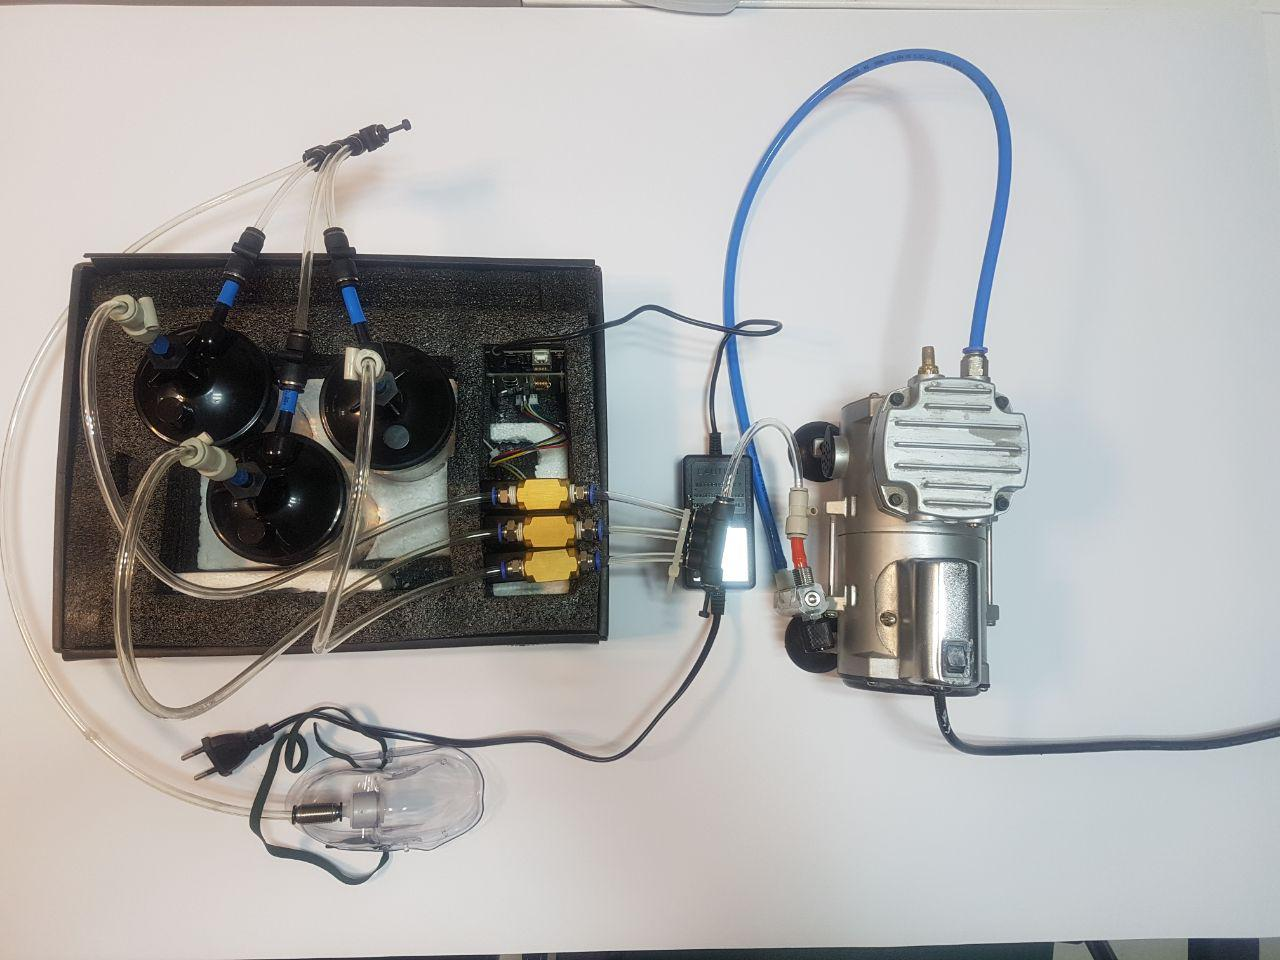
\includegraphics[scale=0.2]{olfactometer.jpg}	
		
	\end{columns}
	
\end{frame}


\begin{frame}
\frametitle{Experimental Protocols}
\begin{enumerate}
	\item
	Task 1: The Oddball Paradigm
	\begin{itemize}
		\item
		two odors and one no-odor control (for resting)
		\item
		one rare and one frequent stimuli
		\item
		rest time: 6s / stimulus time: 4s
		\item
		number of stimuli per trial: 40 / number of trials: 10
		\item
		synchronized respiration (using an auditory or visual stimulus)
	\end{itemize}
	\item
	Task 2: Variable-Length Stimuli
	\begin{itemize}
		\item
		one odor, different durations, and one no-odor control (for resting)
		\item
		rest time: 10s / stimulus time: from 5s to 1min
		\item
		number of stimuli per trial: 10 / number of trials: 10
		\item
		synchronized respiration (using an auditory or visual stimulus)
	\end{itemize}
	
\end{enumerate}
\end{frame}



\begin{frame}
\frametitle{fMRI Data Analysis with SPM}
\begin{figure}
	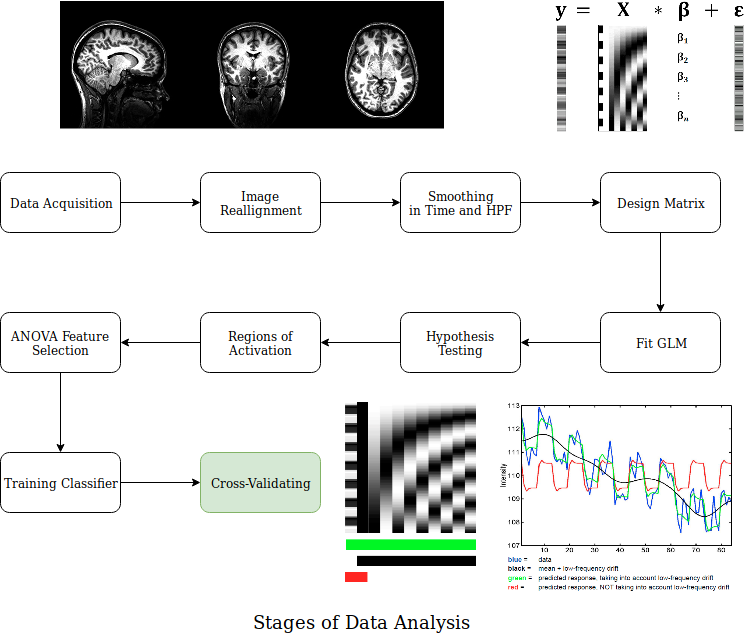
\includegraphics[scale=0.3]{img2.png}
\end{figure}

\end{frame}

\begin{frame}
\frametitle{Project Roadmap}
	\begin{enumerate}
		\item
		Developing a setup for presenting olfactory stimulus \textit{(ALREADY DONE)}
		\item
		finding subjects with olfaction dysfunction
		\item
		fMRI data acquisition
		\item
		data analysis and conclusion (\textit{Estimated Time: 4 months})
	\end{enumerate}

\end{frame}

%----------------------------------------------------------------------------------------

\end{document}